\chapter{Desarrollo reproductor y control de la floración}\label{ch:b2:plant-flowering}

Un cultivador de crisantemos puede hacer florecer un invernadero para
Navidad o para Semana Santa encendiendo o apagando las luces; un trigo de
invierno sembrado en primavera no florece nunca, porque no ha pasado frío;
un cadillo que ha visto una sola noche más larga que su duración crítica
queda comprometido a florecer, pase lo que pase después. Una planta no
tiene calendario, pero tiene relojes, termómetros y fotómetros, y decide
una vez al año, a partir de sus indicaciones, convertir un \omterm{def:b2:plant-meristems:meristem}{meristemo} que
formaba hojas en otro que formará una \omterm{def:b2:angiosperm-reproduction:flower}{flor}. Este capítulo sigue esa
decisión desde la hoja que mide la noche hasta el \omterm{def:b2:plant-meristems:meristem}{meristemo} que cambia de
programa, después la construcción de la \omterm{def:b2:angiosperm-reproduction:flower}{flor} por un código de genes, y la
transición inversa en el otro extremo del ciclo: la \omterm{def:b2:angiosperm-reproduction:seed}{semilla} que no
germina hasta que se le indica que la estación es la adecuada.

\section{La transición a la floración}

\begin{definition}[Transición floral e inducción]\label{def:b2:plant-flowering:transition}
\index{transición floral}\index{inducción floral}\index{meristemo de inflorescencia}
Un \omterm{def:b2:plant-meristems:meristem}{meristemo apical caulinar} vegetativo forma hojas con una yema en cada
axila, indefinidamente. En la \emph{transición floral} se convierte en un
\emph{\omterm{def:b2:plant-meristems:meristem}{meristemo} de inflorescencia}, que forma brácteas y, en sus axilas,
\emph{\omterm{def:b2:plant-meristems:meristem}{meristemos} florales}, cada uno de los cuales es de crecimiento
definido: forma sépalos, pétalos, \omterm{def:b2:angiosperm-reproduction:flower}{estambres} y \omterm{def:b2:angiosperm-reproduction:flower}{carpelos} y después se
detiene. El cambio lo desencadena la \emph{inducción floral} --- una señal
que llega desde las hojas o surge de la propia fisiología de la planta y
que conmuta los genes de identidad del \omterm{def:b2:plant-meristems:meristem}{meristemo}. Las plantas anuales
florecen una vez y mueren; las perennes florecen cada año a partir de
algunos \omterm{def:b2:plant-meristems:meristem}{meristemos} y mantienen otros en estado vegetativo. El momento
decide si el \omterm{def:b2:plant-life-cycles:heterospory}{polen} se encuentra con otro \omterm{def:b2:plant-life-cycles:heterospory}{polen}, si las \omterm{def:b2:angiosperm-reproduction:seed}{semillas} maduran
antes de las heladas y si la \omterm{def:b2:angiosperm-reproduction:flower}{flor} se abre cuando vuela su polinizador:
está sometido a una fuerte selección, y las plantas han desarrollado
varias maneras de leer la estación.
\end{definition}

\begin{proposition}[Fotoperiodismo: la planta mide la noche]\label{prop:b2:plant-flowering:photoperiod}
\index{fotoperiodismo}\index{planta de día corto}\index{planta de día largo}\index{fitocromo}
Muchas plantas florecen en respuesta a la duración del día. Las
\emph{\omterm{prop:b2:plant-flowering:photoperiod}{plantas de día corto}} (crisantemo, soja, arroz, cadillo) florecen
cuando el día es más corto que una duración crítica --- en otoño o en
primavera; las \emph{\omterm{prop:b2:plant-flowering:photoperiod}{plantas de día largo}} (espinaca, trigo, trébol,
\emph{Arabidopsis}), cuando es más largo --- a comienzos del verano; las
plantas \emph{neutras} (tomate, maíz) florecen cuando alcanzan el tamaño
suficiente. Lo que mide la planta es, de hecho, la duración de la
\emph{noche} ininterrumpida: una \omterm{prop:b2:plant-flowering:photoperiod}{planta de día corto} es una planta de
noche larga, y un destello de luz en mitad de una noche larga anula su
efecto, mientras que un periodo de oscuridad en un día largo no lo hace.
La medida se realiza en las \emph{hojas}, mediante el pigmento
\emph{fitocromo} --- una proteína que pasa de una forma que absorbe el rojo
a otra que absorbe el rojo lejano con cada fotón que capta, de modo que
su estado registra la luz ---, confrontado con un \emph{reloj circadiano}
interno de unas veinticuatro horas: la floración se desencadena cuando la
luz coincide con una fase determinada del reloj, lo que solo ocurre con
la duración del día adecuada.
\end{proposition}
\begin{proof}[Evidencia]
Garner y Allard (1920) observaron que un tabaco mutante solo florecía en
los días cortos de un invernadero invernal, y que sojas sembradas a
intervalos durante el verano florecían todas a la vez en septiembre: la
duración del día, y no la edad ni la temperatura, fijaba la fecha. Hamner
y Bonner (1938) mostraron con el cadillo que bastaba una sola noche larga,
que un minuto de luz en mitad de la noche suprimía el efecto y que acortar
el día sin cambiar la noche no inducía la floración. Borthwick y Hendricks
(1952) descubrieron que la luz más eficaz era la roja y que la luz roja
lejana dada inmediatamente después de la roja la anulaba --- la firma del
fitocromo, aislado en 1959. Injertar una sola hoja inducida en una planta
no inducida hacía florecer toda la planta: la hoja exporta una señal.
\end{proof}

\begin{omfigure}
\begin{tikzpicture}[every node/.style={font=\scriptsize}]
  \foreach \y/\lab/\res in {3.6/{día largo, noche corta}/{no florece}, 2.7/{día corto, noche larga}/{florece}, 1.8/{noche larga interrumpida\\por un destello de luz}/{no florece}, 0.9/{día largo interrumpido\\por oscuridad}/{no florece}} {
    \node[anchor=east, align=right] at (-0.2,\y) {\lab};
    \node[anchor=west, omThm] at (8.6,\y) {\res};
  }
  % bars: 24 h = 8 cm; light yellow, dark grey
  \fill[omExo!30] (0,3.4) rectangle (8,3.8); \fill[yellow!50!orange!40] (0,3.4) rectangle (5.4,3.8);
  \fill[omExo!30] (0,2.5) rectangle (8,2.9); \fill[yellow!50!orange!40] (0,2.5) rectangle (3.0,2.9);
  \fill[omExo!30] (0,1.6) rectangle (8,2.0); \fill[yellow!50!orange!40] (0,1.6) rectangle (3.0,2.0); \fill[yellow!50!orange!40] (5.4,1.6) rectangle (5.55,2.0);
  \fill[omExo!30] (0,0.7) rectangle (8,1.1); \fill[yellow!50!orange!40] (0,0.7) rectangle (5.4,1.1); \fill[omExo!30] (2.6,0.7) rectangle (2.9,1.1);
  \draw[thick, ->] (0,0.3) -- (8.2,0.3); \foreach \x/\l in {0/0,2/6,4/12,6/18,8/24} \draw (\x,0.35) -- (\x,0.25) node[below] {\l};
  \node[below] at (4,-0.05) {horas};
  \draw[dashed, omDef] (5.4,0.3) -- (5.4,4.0); \node[omDef, above] at (5.4,4.0) {duración crítica};
\end{tikzpicture}

{\small El cadillo de Hamner y Bonner, una \omterm{prop:b2:plant-flowering:photoperiod}{planta de día corto}. Florece
tras una noche más larga que la duración crítica; un minuto de luz en
mitad de la noche anula la inducción, mientras que un periodo de
oscuridad durante el día no lo hace. La planta mide la noche.}
\end{omfigure}

\begin{definition}[El florígeno]\label{def:b2:plant-flowering:florigen}
\index{florígeno}\index{FLOWERING LOCUS T}
La señal que exporta la hoja recibió el nombre de \emph{florígeno} en
1937 y se identificó setenta años después como una pequeña proteína,
producto del gen \emph{FLOWERING LOCUS T} (FT). En la hoja, el reloj y el
fitocromo activan FT solo cuando la duración del día es la adecuada (en
\emph{Arabidopsis}, una \omterm{prop:b2:plant-flowering:photoperiod}{planta de día largo}, cuando la luz coincide con el
pico vespertino del activador CONSTANS, controlado por el reloj); la
proteína FT entra en el floema, viaja con la corriente de azúcar hasta el
ápice caulinar y allí, con una proteína compañera, activa los genes que
transforman el \omterm{def:b2:plant-meristems:meristem}{meristemo}. La misma proteína es el florígeno del arroz, una
\omterm{prop:b2:plant-flowering:photoperiod}{planta de día corto}, en la que el reloj la conecta al revés. Los
experimentos de injerto, el transporte de la proteína por el floema y la
floración de plantas en las que FT se expresa bajo un promotor específico
de la hoja coinciden: la \omterm{def:b2:angiosperm-reproduction:flower}{flor} se decide en la hoja y se ejecuta en la
yema.
\end{definition}

\begin{omfigure}
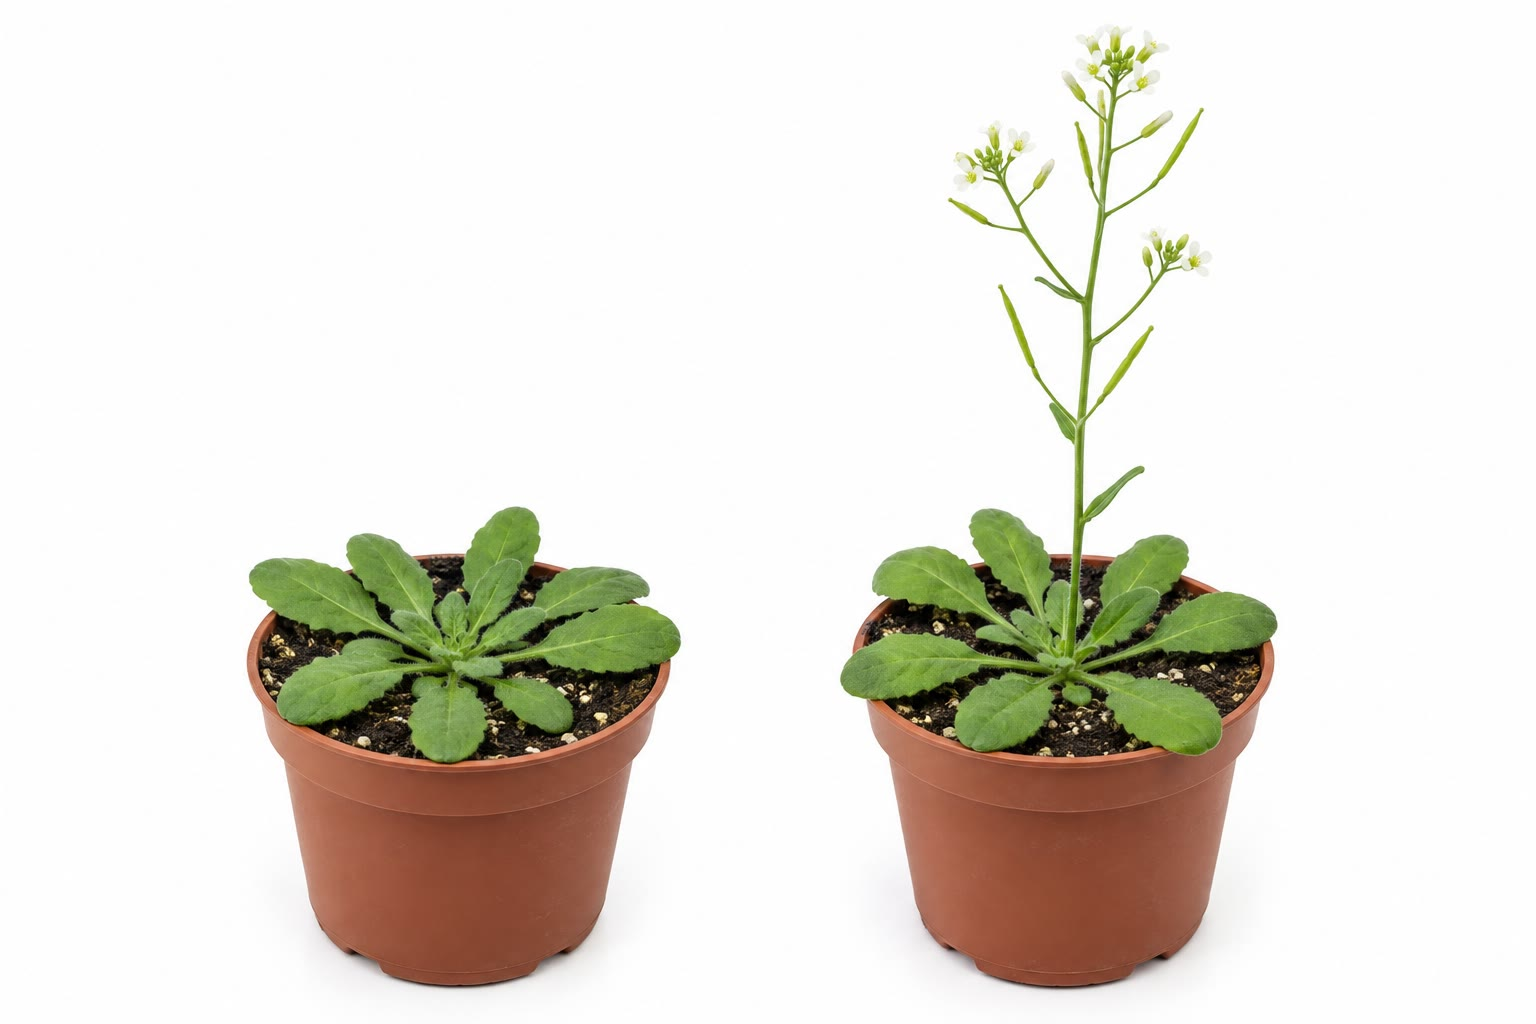
\includegraphics[width=0.58\linewidth]{images/book4/ai/b4-14-arabidopsis-daylength.jpg}

{\small \emph{Arabidopsis}, una \omterm{prop:b2:plant-flowering:photoperiod}{planta de día largo}: en días cortos, una
roseta de hojas; trasladada a días largos, espiga y florece en pocas
semanas.}
\end{omfigure}

\begin{proposition}[La vernalización: la planta cuenta el frío]\label{prop:b2:plant-flowering:vernalisation}
\index{vernalización}\index{FLOWERING LOCUS C}
Los cereales de invierno, las bienales (zanahoria, col, dedalera) y muchas
perennes de climas fríos no florecen hasta haber pasado semanas de frío
--- la \emph{vernalización} ---, lo que garantiza que una planta que
germina en otoño espere a la primavera en lugar de florecer en plenas
heladas. El frío lo percibe el propio \omterm{def:b2:plant-meristems:meristem}{meristemo}, no las hojas; no puede
sustituirse por ningún otro tratamiento; y su efecto se recuerda durante
el resto del crecimiento de la planta, a lo largo de cientos de
divisiones celulares, pero no a través de la \omterm{def:b2:meiosis-heredity:meiosis}{meiosis} --- toda \omterm{def:b2:angiosperm-reproduction:seed}{semilla}
empieza sin vernalizar. En \emph{Arabidopsis} la memoria es un gen,
\emph{\omterm{prop:b2:plant-flowering:vernalisation}{FLOWERING LOCUS C}} (FLC), cuyo producto reprime la floración: semanas
de frío lo silencian progresivamente cubriendo su cromatina de marcas
represoras, el silenciamiento se copia en cada división y se borra en el
embrión. La planta \emph{integra} así el frío a lo largo del tiempo ---
unos pocos días fríos no cuentan ---, y un mutante que carece de FLC no
necesita invierno.
\end{proposition}

\begin{theorem}[Por qué la integración protege frente a una falsa primavera]\label{thm:b2:plant-flowering:integration}
Supóngase que un represor se silencia a un ritmo constante $\alpha$ por
día de frío, de modo que tras $n$ días fríos la fracción todavía activa
es $f_n = e^{-\alpha n}$, y que la floración se permite cuando $f < f_c$.
El número de días fríos necesarios es $n_c = \ln(1/f_c)/\alpha$, y --- como
el silenciamiento es estable --- los días fríos no tienen por qué ser
consecutivos: lo que cuenta es su total. Una planta con $n_c = 40$
días no se deja engañar por dos semanas de deshielo en enero ni por una
ola de frío en octubre; una planta que solo percibiera la temperatura del
momento florecería con la primera semana cálida. La misma integración,
con un umbral, es la manera en que la planta lee la duración del día
acumulada antes de comprometerse; ambas son ejemplos de un sistema que
responde a la \emph{integral} de una señal y no a su valor instantáneo.
\end{theorem}
\begin{proof}
Si cada día frío silencia una fracción $\alpha$ de las copias activas
restantes (o de la cromatina aún sin marcar), la fracción activa cumple
$f_{n+1} = (1 - \alpha)f_n \approx e^{-\alpha}f_n$,
de donde $f_n = e^{-\alpha n}$, con $n$ el número de días fríos; la
desigualdad $e^{-\alpha n} < f_c$ da $n > \ln(1/f_c)/\alpha$. Los días que
no son fríos ni suman ni restan, puesto que las marcas son estables, de
modo que solo importa el total.
\end{proof}

\section{La construcción de la flor: el modelo ABC}

\begin{proposition}[El modelo ABC]\label{prop:b2:plant-flowering:abc}
\index{modelo ABC}\index{gen homeótico!floral}
Un \omterm{def:b2:plant-meristems:meristem}{meristemo} floral dispone cuatro verticilos concéntricos: sépalos,
pétalos, \omterm{def:b2:angiosperm-reproduction:flower}{estambres}, \omterm{def:b2:angiosperm-reproduction:flower}{carpelos}. Sus identidades las fijan tres clases de
\emph{genes homeóticos}, que actúan en anillos solapados: la clase A sola,
en el verticilo 1, da sépalos; A y B juntas, en el verticilo 2, dan
pétalos; B y C juntas, en el verticilo 3, dan \omterm{def:b2:angiosperm-reproduction:flower}{estambres}; C sola, en el
verticilo 4, da \omterm{def:b2:angiosperm-reproduction:flower}{carpelos}. A y C se reprimen mutuamente, de modo que donde
falta una la otra se extiende por toda la \omterm{def:b2:angiosperm-reproduction:flower}{flor}. Las reglas predicen cada
mutante simple: si falta B, la \omterm{def:b2:angiosperm-reproduction:flower}{flor} es sépalo--sépalo--carpelo--carpelo; si
falta C, es sépalo--pétalo--pétalo--sépalo, con otra \omterm{def:b2:angiosperm-reproduction:flower}{flor} dentro, puesto
que C también detiene el \omterm{def:b2:plant-meristems:meristem}{meristemo}; si falta A, es
carpelo--estambre--estambre--carpelo. La mayoría de estos genes codifican
\omterm{prop:b2:cell-differentiation:transcriptional}{factores de transcripción} de una misma familia (MADS-box), y una cuarta
clase, E, es necesaria para las tres funciones; expresar B y C juntas en
una hoja la convierte en un órgano parecido a un \omterm{def:b2:angiosperm-reproduction:flower}{estambre}. Las \omterm{def:b2:angiosperm-reproduction:flower}{flores}
dobles de los jardines --- rosas, peonías, camelias --- son mutantes de la
clase C, con los \omterm{def:b2:angiosperm-reproduction:flower}{estambres} convertidos en pétalos adicionales.
\end{proposition}
\begin{proof}[Evidencia]
Coen y Meyerowitz (1991) compararon los mutantes homeóticos de
\emph{Arabidopsis} y de la boca de dragón: en ambas, tres clases de
\omterm{def:b2:genome-diversification:mutation}{mutaciones} transformaban cada una dos verticilos adyacentes, en los mismos
pares, y las combinaciones de mutantes se comportaban como predice el
modelo (el triple mutante solo forma hojas). La clonación mostró que los
genes eran \omterm{prop:b2:cell-differentiation:transcriptional}{factores de transcripción} expresados en los anillos
predichos; poner un gen B bajo un promotor activo en los cuatro
verticilos dio pétalo--pétalo--estambre--estambre.
\end{proof}

\begin{omfigure}
\begin{tikzpicture}[every node/.style={font=\scriptsize}]
  % four whorls as columns
  \foreach \x/\w in {0/{verticilo 1}, 2.2/{verticilo 2}, 4.4/{verticilo 3}, 6.6/{verticilo 4}} \node[above] at (\x+0.9,3.3) {\w};
  \fill[omDef!35] (0,2.4) rectangle (4.2,3.1); \node at (2.1,2.75) {A};
  \fill[omProp!40] (2.2,1.6) rectangle (6.4,2.3); \node at (4.3,1.95) {B};
  \fill[omThm!30] (4.4,0.8) rectangle (8.6,1.5); \node at (6.5,1.15) {C};
  \foreach \x/\o in {0/sépalos, 2.2/pétalos, 4.4/estambres, 6.6/carpelos} \node[below, align=center] at (\x+0.9,0.6) {\o};
  \node[anchor=west, align=left] at (9.2,3.0) {tipo silvestre: A, AB, BC, C};
  \node[anchor=west, align=left] at (9.2,2.3) {sin B: sépalo, sépalo, carpelo, carpelo};
  \node[anchor=west, align=left] at (9.2,1.6) {sin C: sépalo, pétalo, pétalo, sépalo\ldots};
  \node[anchor=west, align=left] at (9.2,0.9) {sin A: carpelo, estambre, estambre, carpelo};
\end{tikzpicture}

{\small El \omterm{prop:b2:plant-flowering:abc}{modelo ABC}. Tres clases de genes en anillos solapados fijan las
cuatro identidades de órgano; perder una clase transforma dos verticilos,
y las \omterm{def:b2:angiosperm-reproduction:flower}{flores} mutantes son exactamente las predichas.}
\end{omfigure}

\begin{omfigure}
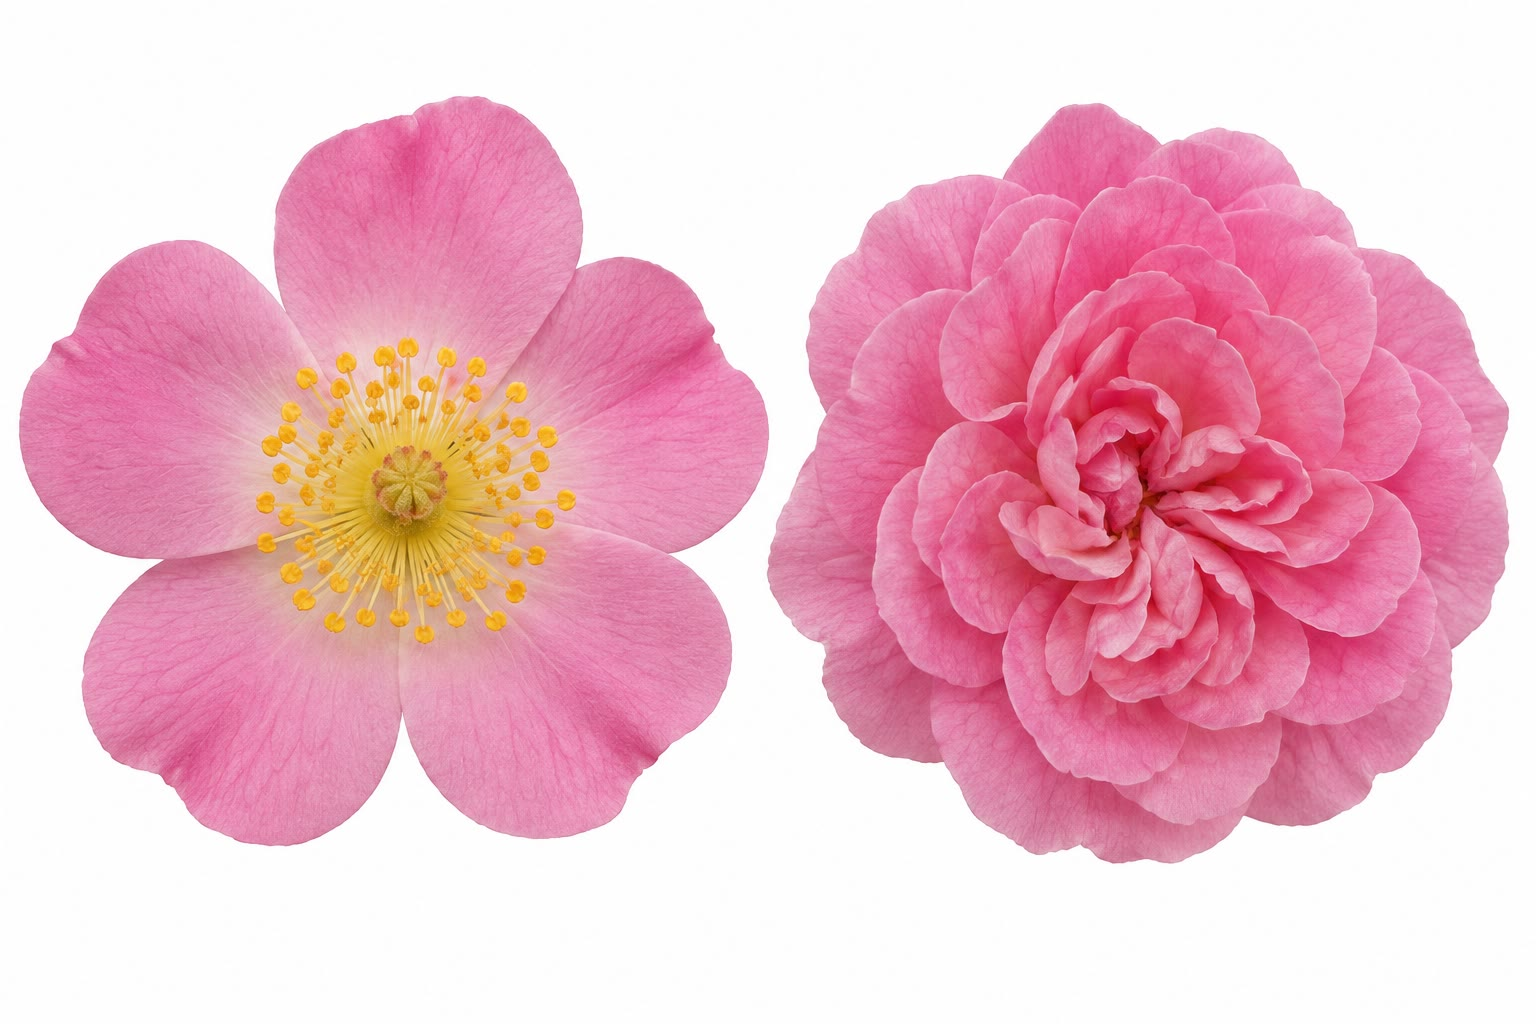
\includegraphics[width=0.58\linewidth]{images/book4/ai/b4-14-double-flower.jpg}

{\small Una \omterm{def:b2:angiosperm-reproduction:flower}{flor} silvestre junto a una forma doble: los \omterm{def:b2:angiosperm-reproduction:flower}{estambres} se han
convertido en pétalos --- un mutante de la clase C, seleccionado por los
jardineros durante siglos antes de que nadie supiera por qué era doble.}
\end{omfigure}

\section{Latencia y germinación}

\begin{definition}[La latencia de las semillas]\label{def:b2:plant-flowering:dormancy}
\index{latencia!de las semillas}\index{ácido abscísico}\index{giberelina}\index{estratificación}
Una \omterm{def:b2:angiosperm-reproduction:seed}{semilla} viable que no germina en condiciones que permitirían el
crecimiento está en \emph{\omterm{def:b2:angiosperm-reproduction:seed}{latencia}}. La \omterm{def:b2:angiosperm-reproduction:seed}{latencia} la impone durante la
maduración de la \omterm{def:b2:angiosperm-reproduction:seed}{semilla} el \emph{ácido abscísico} (ABA), que también
impulsa la acumulación de reservas y la desecación del embrión, y la
mantienen la \omterm{def:b2:angiosperm-reproduction:seed}{cubierta seminal} (impermeable al agua o al oxígeno, o que
restringe mecánicamente) o el propio estado del embrión. La rompen las
señales que marcan el final de la estación desfavorable: semanas de frío
y humedad (la \emph{estratificación}, la vernalización de la \omterm{def:b2:angiosperm-reproduction:seed}{semilla}), la
luz --- en las \omterm{def:b2:angiosperm-reproduction:seed}{semillas} pequeñas que deben estar cerca de la superficie,
percibida por el fitocromo --- o la oscuridad, las temperaturas
alternas, el lavado de inhibidores por la lluvia, la escarificación de la
cubierta por el suelo o por un tubo digestivo, el humo y el calor tras un
incendio. La decisión es un equilibrio entre el ABA y la
\emph{giberelina}: las señales que rompen la \omterm{def:b2:angiosperm-reproduction:seed}{latencia} reducen el ABA y
elevan la giberelina, que moviliza las reservas
(\cref{ch:b2:angiosperm-reproduction}) y permite crecer a la radícula. Una
población de \omterm{def:b2:angiosperm-reproduction:seed}{semillas} no es uniforme: una fracción germina a la primera
oportunidad y el resto espera un año o más, de modo que ninguna mala
estación aislada acaba con toda la cohorte --- el \emph{banco de
\omterm{def:b2:angiosperm-reproduction:seed}{semillas}}, una cobertura frente a un mundo impredecible.
\end{definition}
\begin{proof}[Evidencia]
Las \omterm{def:b2:angiosperm-reproduction:seed}{semillas} de lechuga (Borthwick, 1952) germinan en la oscuridad tras un
destello de luz roja y no tras un destello de rojo lejano; si reciben
rojo, después rojo lejano y después rojo, germinan --- decide el último
destello. El mismo pigmento reversible que sincroniza la floración pone
en marcha la germinación. Las \omterm{def:b2:angiosperm-reproduction:seed}{semillas} de muchos árboles sembradas recién
recogidas en suelo cálido no hacen nada; las mismas \omterm{def:b2:angiosperm-reproduction:seed}{semillas}, tras dos
meses en un frigorífico húmedo, germinan de inmediato, y los mutantes
deficientes en ABA germinan sobre la planta antes incluso de que la
\omterm{def:b2:angiosperm-reproduction:seed}{semilla} se seque.
\end{proof}

\begin{omfigure}
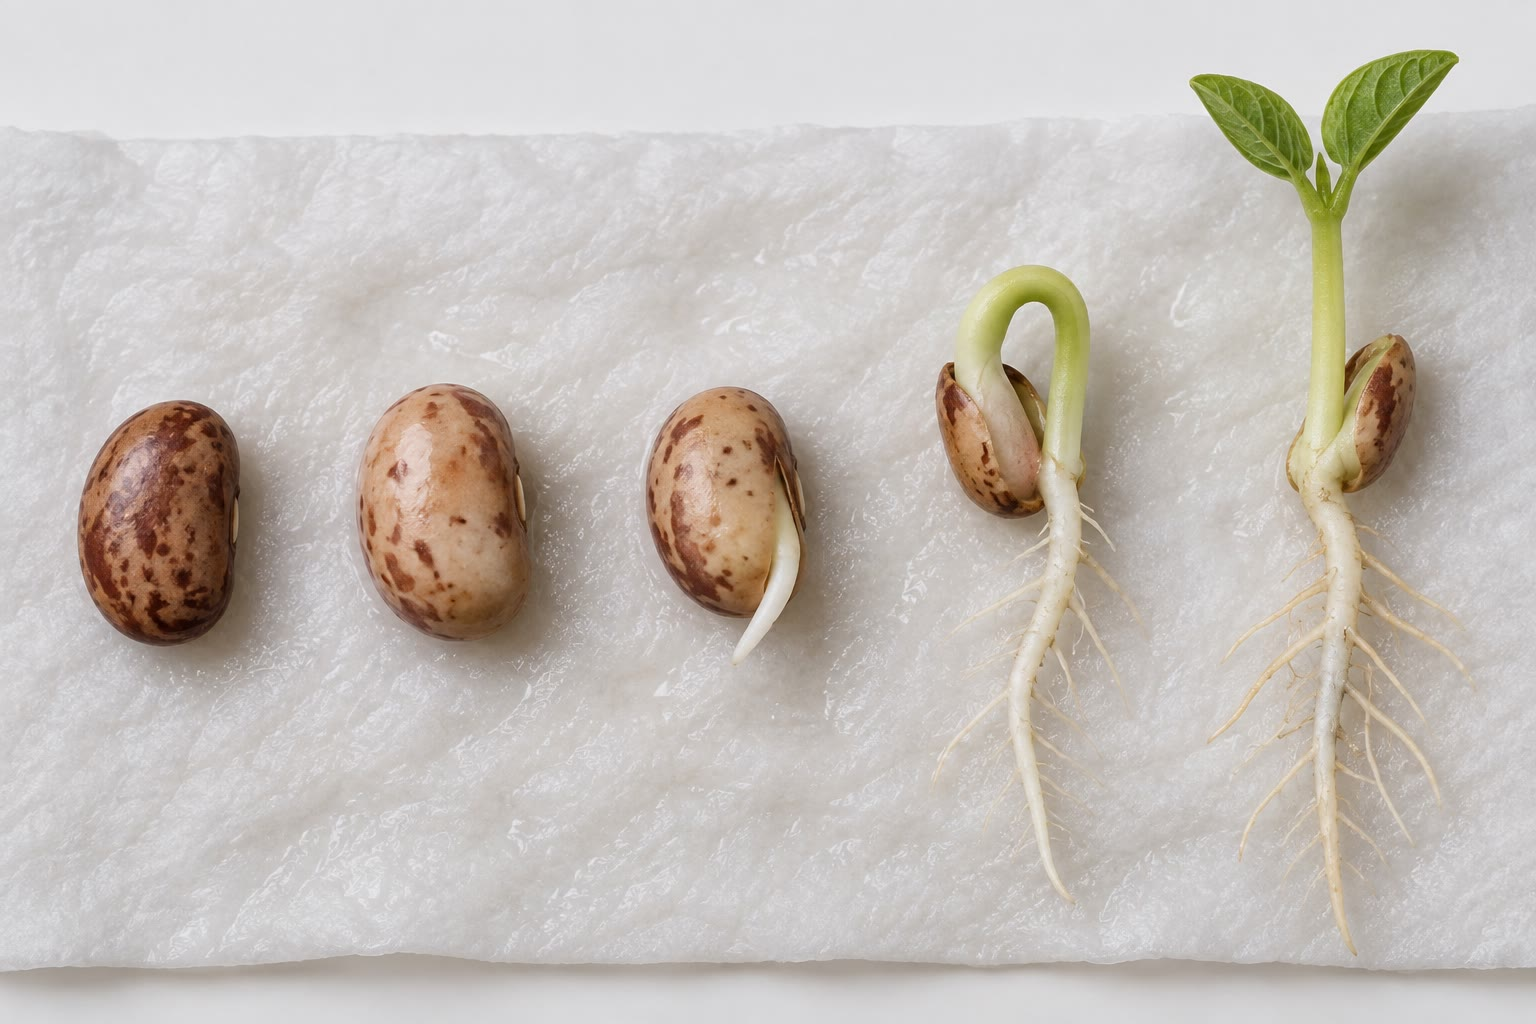
\includegraphics[width=0.66\linewidth]{images/book4/ai/b4-14-germinating-beans.jpg}

{\small La germinación de la judía: la \omterm{def:b2:angiosperm-reproduction:seed}{semilla} se embebe, la radícula sale
primero, el hipocótilo se abre paso a través del suelo en forma de gancho,
y el gancho se endereza a la luz mientras se abren las primeras hojas.}
\end{omfigure}

\begin{theorem}[La germinación como apuesta]\label{thm:b2:plant-flowering:bet}
\index{diversificación del riesgo}
Sea $g$ la fracción de una cohorte de \omterm{def:b2:angiosperm-reproduction:seed}{semillas} que germina cada año, y
supóngase que el resto sobrevive en el suelo hasta el año siguiente con
probabilidad $s$. En un buen año, una \omterm{def:b2:angiosperm-reproduction:seed}{semilla} que germina deja $R_g$
\omterm{def:b2:angiosperm-reproduction:seed}{semillas}; en un mal año, ninguna; los años son buenos con probabilidad
$p$. Una estrategia que lo hace germinar todo a la vez ($g = 1$) tiene, a
lo largo de una serie de años, una tasa de crecimiento a largo plazo
promediada en $\ln$ igual a $p\ln R_g + (1 - p)\ln 0 =
-\infty$: un solo mal año la extingue. Una estrategia con $g < 1$
crece en los buenos años en un factor $gR_g + (1 - g)s$ y en los malos
en un factor $(1 - g)s > 0$, de modo que su tasa a largo plazo,
\[
r = p\ln\bigl(gR_g + (1 - g)s\bigr) + (1 - p)\ln\bigl((1 - g)s\bigr),
\]
es finita y, para $p$ no demasiado próxima a 1, alcanza su máximo en un
$g$ intermedio. Con $R_g = 20$, $s = 0.8$ y $p = 0.7$, el óptimo está
cerca de $g = 0.7$: germinar la mayoría y guardar una reserva. La \omterm{def:b2:angiosperm-reproduction:seed}{latencia}
no es un fracaso de la germinación, sino un rechazo parcial seleccionado
por la evolución.
\end{theorem}
\begin{proof}
El tamaño de la población al cabo de $T$ años es el producto de los
factores anuales, de modo que su tasa de crecimiento es la media de sus
logaritmos (la tasa media geométrica), que es lo que maximiza la
selección en series largas. Con $g = 1$ el factor de los malos años es
cero y su logaritmo es $-\infty$. Para $g < 1$ ambos factores son
positivos; derivando $r$ respecto a $g$ e igualando a cero se obtiene el
óptimo, que para las cifras citadas se sitúa cerca de $g = 0.7$
(evaluar $r$ en $g = 0.4, 0.6, 0.8, 1$ da $1.28$, $1.42$,
$1.40$, $-\infty$).
\end{proof}

\begin{omfigure}
\begin{tikzpicture}
\begin{axis}[
  width=0.7\linewidth, height=5.4cm,
  axis x line=bottom, axis y line=left,
  xmin=0, xmax=1, ymin=0, ymax=1.7,
  xlabel={fracción que germina cada año, $g$}, ylabel={tasa de crecimiento a largo plazo $r$},
  xlabel style={font=\small, at={(axis description cs:0.5,-0.13)}, anchor=north},
  ylabel style={font=\small},
  tick label style={font=\small}, xtick={0,0.2,0.4,0.6,0.8,1}, ytick={0,0.5,1,1.5},
  clip=false,
]
\addplot[very thick, omDef, domain=0.02:0.97, samples=100] {0.7*ln(20*x + 0.8*(1-x)) + 0.3*ln(0.8*(1-x))};
\draw[dashed, gray] (axis cs:0.7,0) -- (axis cs:0.7,1.43);
\node[font=\scriptsize, anchor=south] at (axis cs:0.7,1.45) {óptimo: guardar un \qty{30}{\%} en el suelo};
\node[font=\scriptsize, anchor=north west, align=left] at (axis cs:0.7,0.6) {$g \to 1$: un solo mal año\\acaba con la cohorte};
\end{axis}
\end{tikzpicture}

{\small La \omterm{thm:b2:plant-flowering:bet}{diversificación del riesgo} mediante la \omterm{def:b2:angiosperm-reproduction:seed}{latencia}. Con años
buenos siete de cada diez, una cohorte que germina entera acaba destruida
por un mal año; una cohorte que retiene una parte de sus \omterm{def:b2:angiosperm-reproduction:seed}{semillas} crece
más deprisa a largo plazo.}
\end{omfigure}

\section{Ejercicios}

\begin{exercise}[$\star$]\label{exo:b2:plant-flowering:1}
Distíngase entre \omterm{def:b2:plant-meristems:meristem}{meristemos} vegetativos, de inflorescencia y florales, y
dígase cuáles son de crecimiento definido.
\end{exercise}

\begin{exercise}[$\star$]\label{exo:b2:plant-flowering:2}
Defínanse las \omterm{prop:b2:plant-flowering:photoperiod}{plantas de día corto}, de día largo y neutras con un ejemplo
de cada una, y dígase qué mide en realidad una \omterm{prop:b2:plant-flowering:photoperiod}{planta de día corto}.
\end{exercise}

\begin{exercise}[$\star$]\label{exo:b2:plant-flowering:3}
Dese la identidad de órgano de cada verticilo en el tipo silvestre y en
los tres mutantes simples del \omterm{prop:b2:plant-flowering:abc}{modelo ABC}.
\end{exercise}

\begin{exercise}[$\star$]\label{exo:b2:plant-flowering:4}
Nómbrense cuatro señales que rompen la \omterm{def:b2:angiosperm-reproduction:seed}{latencia} de las \omterm{def:b2:angiosperm-reproduction:seed}{semillas} y, para
cada una, la estación o el lugar que indica.
\end{exercise}

\begin{exercise}[$\star\star$]\label{exo:b2:plant-flowering:5}
Una \omterm{prop:b2:plant-flowering:photoperiod}{planta de día corto} tiene una noche crítica de \qty{10}{h}. Dígase si
florece con: \qty{16}{h} de luz/\qty{8}{h} de oscuridad; \qty{12}{h}/\qty{12}{h};
\qty{12}{h} de luz, \qty{6}{h} de oscuridad, un minuto de luz, \qty{6}{h} de oscuridad;
\qty{8}{h} de luz, \qty{4}{h} de oscuridad, \qty{4}{h} de luz, \qty{8}{h} de oscuridad.
\end{exercise}

\begin{exercise}[$\star\star$]\label{exo:b2:plant-flowering:6}
Una hoja de una \omterm{prop:b2:plant-flowering:photoperiod}{planta de día corto} inducida se injerta en una \omterm{prop:b2:plant-flowering:photoperiod}{planta de
día largo} mantenida en días largos, y la \omterm{prop:b2:plant-flowering:photoperiod}{planta de día largo} florece.
¿Qué muestra esto sobre el \omterm{def:b2:plant-flowering:florigen}{florígeno}? ¿Y si el injerto se hace con una
hoja inducida cuyo floema está interrumpido en el pecíolo?
\end{exercise}

\begin{exercise}[$\star\star$]\label{exo:b2:plant-flowering:7}
El frío silencia el represor con $\alpha = 0.05$ por día y la floración
requiere $f < 0.15$. ¿Cuántos días fríos hacen falta? Un invierno tiene
tres periodos fríos de 15, 12 y 20 días separados por deshielos: ¿queda
vernalizada la planta? ¿Y si $\alpha$ fuera $0.02$?
\end{exercise}

\begin{exercise}[$\star\star$]\label{exo:b2:plant-flowering:8}
Explíquese, en términos de cromatina, por qué la memoria de una planta
vernalizada se pierde en sus \omterm{def:b2:angiosperm-reproduction:seed}{semillas}, y por qué esto es útil.
\end{exercise}

\begin{exercise}[$\star\star$]\label{exo:b2:plant-flowering:9}
Unas \omterm{def:b2:angiosperm-reproduction:seed}{semillas} de lechuga reciben, en la oscuridad, las secuencias: R; R y
después RL; R, RL, R; R, RL, R, RL. Predígase la germinación en cada caso
y explíquese en términos de las dos formas del fitocromo.
\end{exercise}

\begin{exercise}[$\star\star\star$]\label{exo:b2:plant-flowering:10}
En el modelo de \omterm{thm:b2:plant-flowering:bet}{diversificación del riesgo} con $R_g = 20$ y $s = 0.8$,
calcúlese la tasa de crecimiento a largo plazo para $g = 0.4$, $0.6$,
$0.8$ y $1$ cuando $p = 0.7$, y de nuevo cuando $p = 0.95$. ¿Cómo se
desplaza el óptimo, y qué predice esto para los desiertos frente a las
praderas?
\end{exercise}

\begin{exercise}[$\star\star\star$]\label{exo:b2:plant-flowering:11}
Predígase la \omterm{def:b2:angiosperm-reproduction:flower}{flor} producida al expresar un gen de la clase B en los cuatro
verticilos; al expresar la clase C en los cuatro; en un doble mutante que
carece de A y de B. Explíquese después por qué la \omterm{def:b2:angiosperm-reproduction:flower}{flor} sin C sigue
formando verticilos.
\end{exercise}

\begin{exercise}[$\star\star\star$]\label{exo:b2:plant-flowering:12}
``Una planta decide florecer integrando señales que no puede controlar.''
Discútanse las tres integraciones de este capítulo --- de la duración del
día, del frío y de los años en el banco de \omterm{def:b2:angiosperm-reproduction:seed}{semillas} --- y de qué protege
a la planta un integrador que un simple umbral no protegería.
\end{exercise}

\section{Problema: el calendario del cultivador}

\begin{problem}[{Problema de fin de semana --- un cultivador de
crisantemos programa la floración con luces, un mejorador de trigo cuenta
el frío, se explica la flor doble de un florista y se modeliza la latencia
de un lote de semillas, hasta llegar a la duración de la noche que
desencadena el cultivo, los días de frío que necesita el trigo y la mejor
fracción de germinación}]
\label{pb:b2:plant-flowering:1}
El crisantemo es una \omterm{prop:b2:plant-flowering:photoperiod}{planta de día corto} con una duración crítica de la
noche de \qty{9.5}{h}; la inducción requiere \num{12} noches inductivas
consecutivas, y las \omterm{def:b2:angiosperm-reproduction:flower}{flores} se abren \num{8} semanas después de la
inducción. En noviembre el invernadero está a oscuras de 17:00 a 07:30.
El trigo de invierno tiene $\alpha = 0.06$ por día frío y florece cuando
$f < 0.10$. Lote de \omterm{def:b2:angiosperm-reproduction:seed}{semillas}: $R_g = 15$, $s = 0.7$, años buenos con
probabilidad $p$.

\medskip
\noindent\textbf{Parte I --- El invernadero.}
\begin{enumerate}
  \item En junio la noche natural dura \qty{8}{h}. ¿Florecerá el cultivo?
        ¿Qué debe hacer el cultivador para vender \omterm{def:b2:angiosperm-reproduction:flower}{flores} en agosto?
  \item El cultivador cubre el cultivo con una tela negra de 19:00 a
        07:00. ¿Qué duración de la noche percibe la planta, y cuándo debe
        empezar a cubrirlo para que florezca el 15~de agosto?
  \item En noviembre la noche natural dura \qty{14}{h} y el cultivador
        quiere \emph{retrasar} la floración hasta Navidad. Propóngase un
        programa de iluminación y explíquese por qué basta un breve
        destello.
  \item El destello se da a las 21:00 en lugar de a las 00:00, y la
        inducción no se impide. Explíquese con la duración crítica de la
        noche.
  \item Una noche de las doce, la tela se queda sin poner. Predígase el
        resultado, y dígase qué habría hecho un cadillo.
  \item El destello se da con luz verde y fracasa; con luz roja funciona;
        rojo seguido de rojo lejano fracasa. Explíquese.
  \item Se injerta una sola hoja de una planta inducida en una planta en
        días largos. Predígase el resultado, y dígase qué identifica.
\end{enumerate}

\medskip
\noindent\textbf{Parte II --- El trigo.}
\begin{enumerate}[resume]
  \item ¿Cuántos días fríos necesita el trigo?
  \item Sembrado en octubre, recibe 10 días fríos en noviembre, un
        diciembre suave, 25 en enero y 12 en febrero. ¿Cuándo queda
        vernalizado?
  \item Sembrado en marzo, recibe 6 días fríos. ¿Florece ese verano? ¿Qué
        consecuencia agrícola tiene?
  \item Un mutante carece del represor. Predígase su comportamiento y
        dígase por qué los mejoradores llaman a esos trigos ``trigos de
        primavera''.
  \item Explíquese por qué la memoria del frío sobrevive a las divisiones
        del \omterm{def:b2:plant-meristems:meristem}{meristemo} a lo largo de la primavera, pero no a la \omterm{def:b2:meiosis-heredity:meiosis}{meiosis} que
        forma la generación siguiente.
  \item ¿Por qué el frío debe contarse en el \omterm{def:b2:plant-meristems:meristem}{meristemo} y no en las hojas, a
        diferencia de la duración del día?
\end{enumerate}

\medskip
\noindent\textbf{Parte III --- El florista.}
\begin{enumerate}[resume]
  \item Una rosa doble tiene pétalos donde deberían estar los \omterm{def:b2:angiosperm-reproduction:flower}{estambres} y
        unos pocos pétalos adicionales en el centro. ¿Qué clase de gen ha
        fallado? Dese la fórmula de los verticilos.
  \item Esas rosas son estériles como progenitoras de \omterm{def:b2:plant-life-cycles:heterospory}{polen}, pero a veces
        forman \omterm{def:b2:angiosperm-reproduction:seed}{semillas}. Explíquense ambos hechos a partir del \omterm{prop:b2:plant-flowering:abc}{modelo ABC}.
  \item Una boca de dragón tiene \omterm{def:b2:angiosperm-reproduction:flower}{estambres} en lugar de pétalos y \omterm{def:b2:angiosperm-reproduction:flower}{carpelos}
        en lugar de sépalos. ¿Qué clase ha fallado?
  \item Predígase la \omterm{def:b2:angiosperm-reproduction:flower}{flor} de una planta en la que la clase C se expresa
        también en el verticilo 1, además de en sus verticilos normales.
  \item ¿Por qué las mismas \omterm{def:b2:genome-diversification:mutation}{mutaciones} produjeron las mismas
        transformaciones en una rosa, una boca de dragón y
        \emph{Arabidopsis}, plantas separadas por cien millones de años?
  \item En el verticilo 2 de una \omterm{def:b2:angiosperm-reproduction:flower}{flor} silvestre están activas A y B.
        Predígase el órgano si solo estuviera activa B.
\end{enumerate}

\medskip
\noindent\textbf{Parte IV --- El lote de \omterm{def:b2:angiosperm-reproduction:seed}{semillas}.}
\begin{enumerate}[resume]
  \item Calcúlese la tasa de crecimiento a largo plazo $r$ para $g = 0.5$,
        $0.7$ y $0.9$ cuando $p = 0.8$.
  \item ¿Cuál de las tres es la mejor? ¿Qué ocurre con $g = 1$?
  \item Vuélvase a calcular para $p = 0.5$ (un desierto). ¿Qué $g$ es ahora
        el mejor?
  \item Un cultivador siembra todo el lote en un campo en un buen año y
        cosecha $R_g$ por \omterm{def:b2:angiosperm-reproduction:seed}{semilla}. Explíquese por qué su estrategia difiere
        de la de la planta y qué debe hacer para conservar la variedad a
        lo largo de un mal año.
  \item Las \omterm{def:b2:angiosperm-reproduction:seed}{semillas} necesitan luz para germinar. Explíquese el sentido
        adaptativo de esto para una \omterm{def:b2:angiosperm-reproduction:seed}{semilla} pequeña, y predígase qué le
        hace el arado al banco de \omterm{def:b2:angiosperm-reproduction:seed}{semillas}.
  \item Enúnciese el resultado: la duración crítica de la noche y el
        programa de cubrición, la necesidad de frío del trigo y el mejor
        $g$ para $p = 0.8$ y para $p = 0.5$.
\end{enumerate}
\end{problem}
